%%%%%%%%%%%%%%%%%%%%%%%%%%%%%%%%%%%%%%%%
% Programming/Coding Assignment
% LaTeX Template
%
% Original author:
% Ted Pavlic (http://www.tedpavlic.com)
%
%
% This template uses a Perl script as an example snippet of code, most other
% languages are also usable. Configure them in the "CODE INCLUSION 
% CONFIGURATION" section.
%
%%%%%%%%%%%%%%%%%%%%%%%%%%%%%%%%%%%%%%%%%

%----------------------------------------------------------------------------------------
%	PACKAGES AND OTHER DOCUMENT CONFIGURATIONS
%----------------------------------------------------------------------------------------

\documentclass{article}
\usepackage[latin1]{inputenc}

\usepackage[english]{babel}
\usepackage{amsmath}
\usepackage{amssymb}
\usepackage{mathtools}
\usepackage{amsfonts}
\usepackage{fancyhdr} % Required for custom headers
\usepackage{lastpage} % Required to determine the last page for the footer
\usepackage{extramarks} % Required for headers and footers
\usepackage[usenames,dvipsnames]{color} % Required for custom colors
\usepackage{graphicx} % Required to insert images
\usepackage{listings} % Required for insertion of code
\usepackage{courier} % Required for the courier font
\usepackage{enumerate} % used for enumerate args
\usepackage{multicol} % columns

\usepackage{pgf} 
\usepackage{tikz}
\usepackage{forest} % treees :D
\usetikzlibrary{arrows,automata} %for FSM

% Custom commands
\DeclareMathOperator{\Kl}{Kl} %Klassen von Zuständen

\usepackage{mathtools}
\DeclarePairedDelimiter{\ceil}{\lceil}{\rceil}
% Shamelessly copied from http://tex.stackexchange.com/questions/43008/absolute-value-symbols
\DeclarePairedDelimiter\abs{\lvert}{\rvert} % nice |x|
\DeclarePairedDelimiter\norm{\lVert}{\rVert} % nice ||x||
% Swap the definition of \abs* and \norm*, so that \abs
% and \norm resizes the size of the brackets, and the 
% starred version does not.
\makeatletter
\let\oldabs\abs
\def\abs{\@ifstar{\oldabs}{\oldabs*}}
\let\oldnorm\norm
\def\norm{\@ifstar{\oldnorm}{\oldnorm*}}
\makeatother


% Margins
\topmargin=-0.45in
\evensidemargin=0in
\oddsidemargin=0in
\textwidth=6.5in
\textheight=9.0in
\headsep=0.25in

\linespread{1.1} % Line spacing

% Set up the header and footer
\pagestyle{fancy}
\lhead{\hmwkAuthorName} % Top left header
%\chead{\hmwkClass\ (\hmwkClassInstructor\): \hmwkTitle} % Top center head
%\rhead{\firstxmark} % Top right header
\rhead{}
\lfoot{\lastxmark} % Bottom left footer
\cfoot{} % Bottom center footer
\rfoot{Seite\ \thepage\ von\ \protect\pageref{LastPage}} % Bottom right footer
\renewcommand\headrulewidth{0.4pt} % Size of the header rule
\renewcommand\footrulewidth{0.4pt} % Size of the footer rule

\setlength\parindent{0pt} % Removes all indentation from paragraphs

%----------------------------------------------------------------------------------------
%	CODE INCLUSION CONFIGURATION
%----------------------------------------------------------------------------------------

\definecolor{MyDarkGreen}{rgb}{0.0,0.4,0.0} % This is the color used for comments
\lstloadlanguages{Pascal} % Load Pascal syntax for listings, for a list of other languages supported see: ftp://ftp.tex.ac.uk/tex-archive/macros/latex/contrib/listings/listings.pdf
\lstset{language=Perl, % Use Pascal in this example
        frame=single, % Single frame around code
        basicstyle=\small\ttfamily, % Use small true type font
        keywordstyle=[1]\color{Blue}\bf, % Pascal functions bold and blue
        keywordstyle=[2]\color{Purple}, % Pascal function arguments purple
        keywordstyle=[3]\color{Blue}\underbar, % Custom functions underlined and blue
        identifierstyle=, % Nothing special about identifiers                                         
        commentstyle=\usefont{T1}{pcr}{m}{sl}\color{MyDarkGreen}\small, % Comments small dark green courier font
        stringstyle=\color{Purple}, % Strings are purple
        showstringspaces=false, % Don't put marks in string spaces
        tabsize=5, % 5 spaces per tab
        %
        % Put standard Pascal functions not included in the default language here
        morekeywords={rand},
        %
        % Put Pascal function parameters here
        morekeywords=[2]{on, off, interp},
        %
        % Put user defined functions here
        morekeywords=[3]{test},
        %
        morecomment=[l][\color{Blue}]{...}, % Line continuation (...) like blue comment
        numbers=left, % Line numbers on left
        firstnumber=1, % Line numbers start with line 1
        numberstyle=\tiny\color{Blue}, % Line numbers are blue and small
        stepnumber=5 % Line numbers go in steps of 5
}

% Creates a new command to include a perl script, the first parameter is the filename of the script (without .p), the second parameter is the caption
\newcommand{\pascalscript}[2]{
\begin{itemize}
\item[]\lstinputlisting[caption=#2,label=#1]{#1.p}
\end{itemize}
}

%----------------------------------------------------------------------------------------
%	DOCUMENT STRUCTURE COMMANDS
%	Skip this unless you know what you're doing
%----------------------------------------------------------------------------------------

% Header and footer for when a page split occurs within a problem environment
%\newcommand{\enterProblemHeader}[1]{
%\nobreak\extramarks{#1}{#1 continued on next page\ldots}\nobreak
%\nobreak\extramarks{#1 (continued)}{#1 continued on next page\ldots}\nobreak
%}

% Header and footer for when a page split occurs between problem environments
%\newcommand{\exitProblemHeader}[1]{
%\nobreak\extramarks{#1 (continued)}{#1 continued on next page\ldots}\nobreak
%\nobreak\extramarks{#1}{}\nobreak
%}

\setcounter{secnumdepth}{0} % Removes default section numbers
\newcounter{homeworkProblemCounter} % Creates a counter to keep track of the number of problems

\newcommand{\homeworkProblemName}{}
\newenvironment{homeworkProblem}[1][Aufgabe \arabic{homeworkProblemCounter}]{ % Makes a new environment called homeworkProblem which takes 1 argument (custom name) but the default is "Problem #"
\stepcounter{homeworkProblemCounter} % Increase counter for number of problems
\renewcommand{\homeworkProblemName}{#1} % Assign \homeworkProblemName the name of the problem
\section{\homeworkProblemName} % Make a section in the document with the custom problem count
%\enterProblemHeader{\homeworkProblemName} % Header and footer within the environment
}{
%\exitProblemHeader{\homeworkProblemName} % Header and footer after the environment
}

\newcommand{\problemAnswer}[1]{ % Defines the problem answer command with the content as the only argument
\noindent\framebox[\columnwidth][c]{\begin{minipage}{0.98\columnwidth}#1\end{minipage}} % Makes the box around the problem answer and puts the content inside
}

\newcommand{\homeworkSectionName}{}
\newenvironment{homeworkSection}[1]{ % New environment for sections within homework problems, takes 1 argument - the name of the section
\renewcommand{\homeworkSectionName}{#1} % Assign \homeworkSectionName to the name of the section from the environment argument
\subsection{\homeworkSectionName} % Make a subsection with the custom name of the subsection
%\enterProblemHeader{\homeworkProblemName\ [\homeworkSectionName]} % Header and footer within the environment
}{
%\enterProblemHeader{\homeworkProblemName} % Header and footer after the environment
}

%----------------------------------------------------------------------------------------
%	NAME AND CLASS SECTION
%----------------------------------------------------------------------------------------

\newcommand{\hmwkTitle}{Blatt} % Assignment title
\newcommand{\hmwkDueDate}{9.\ Oktober\ 2015} % Due date
\newcommand{\hmwkClass}{Theoretische Informatik} % Course/class
\newcommand{\hmwkClassInstructor}{} % Teacher/lecturer
\newcommand{\hmwkAuthorName}{Linus Fessler, Markus Hauptner, Philipp Schimmelfennig} % Your name
\newcommand{\hmwkNumber}{1}

%----------------------------------------------------------------------------------------
%	TITLE PAGE
%----------------------------------------------------------------------------------------

\title{
\vspace{2in}
\textmd{\textbf{\hmwkClass:\ \hmwkTitle\ \hmwkNumber}}\\
\normalsize\vspace{0.1in}\small{Abgabe\ bis\ \hmwkDueDate}
\\Assistent: Sascha Krug, CHN D 42
\\
\vspace{0.1in}\large{\textit{\hmwkClassInstructor}
\vspace{3in}
}}
\author{\textbf{\hmwkAuthorName}}
\date{} % Insert date here if you want it to appear below your name

%----------------------------------------------------------------------------------------

\begin{document}

\maketitle

%----------------------------------------------------------------------------------------
%	TABLE OF CONTENTS
%----------------------------------------------------------------------------------------

%\setcounter{tocdepth}{1} % Uncomment this line if you don't want subsections listed in the ToC

\addtocounter{homeworkProblemCounter}{0}
\newpage
%\tableofcontents
%\newpage

%----------------------------------------------------------------------------------------
%	Aufgabe S1
%----------------------------------------------------------------------------------------

\begin{homeworkProblem}
\begin{enumerate}[(a)]

\item
Der nachstehende endliche Automat akzeptiert nur Wörter der Sprache $L_1=\{w \in \{a,b\}^* \mid (2 \cdot |w|_a - |w|_b + 1)\text{ mod }5 = 2\}.$

\begin{center}
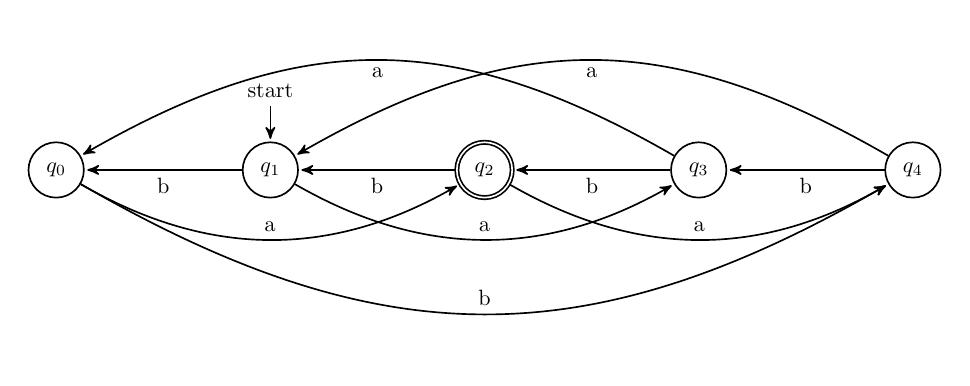
\begin{tikzpicture}[->,>=stealth',shorten >=1pt,auto,node distance=3.4cm,
                    semithick,every node/.style={scale=0.8}]
  \tikzstyle{every state}=[circle,text=black]

  \node[state] 				(A)             	{$q_0$};
  \node[initial above,state](B) [right of=A]	{$q_1$};
  \node[state,accepting]	(C) [right of=B]	{$q_2$};
  \node[state]        		(D) [right of=C]	{$q_3$};
  \node[state]        		(E) [right of=D]	{$q_4$};

  \path (A)	edge [bend right]				node {a} (C)
  			edge [bend right,looseness=1.1]	node {b} (E)
  		(B)	edge [bend right]				node {a} (D)
			edge							node {b} (A)
  		(C)	edge [bend right]				node {a} (E)
  			edge 							node {b} (B)
  		(D)	edge [bend right,looseness=1.1]	node {a} (A)
  			edge 							node {b} (C)
  		(E)	edge [bend right,looseness=1.1]	node {a} (B)
  			edge 							node {b} (D)
  ;
\end{tikzpicture}
\end{center}

Die Klassen seiner Zustände sind:
\begin{enumerate}[\quad]
\item Kl[$q_0$] = $\{w \in \{a,b\}^* \mid (2 \cdot |w|_a - |w|_b + 1)\text{ mod }5 = 0\}$
\item Kl[$q_1$] = $\{w \in \{a,b\}^* \mid (2 \cdot |w|_a - |w|_b + 1)\text{ mod }5 = 1\}$
\item Kl[$q_2$] = $\{w \in \{a,b\}^* \mid (2 \cdot |w|_a - |w|_b + 1)\text{ mod }5 = 2\}$
\item Kl[$q_3$] = $\{w \in \{a,b\}^* \mid (2 \cdot |w|_a - |w|_b + 1)\text{ mod }5 = 3\}$
\item Kl[$q_4$] = $\{w \in \{a,b\}^* \mid (2 \cdot |w|_a - |w|_b + 1)\text{ mod }5 = 4\}$
\end{enumerate}

\item
Folgender endlicher Automat akzeptiert nur Wörter der Sprache $L_2=\{bbxa \mid x \in \{a,b\}^*$ und $x$ enthält das Teilwort $aa\}$.

\begin{center}
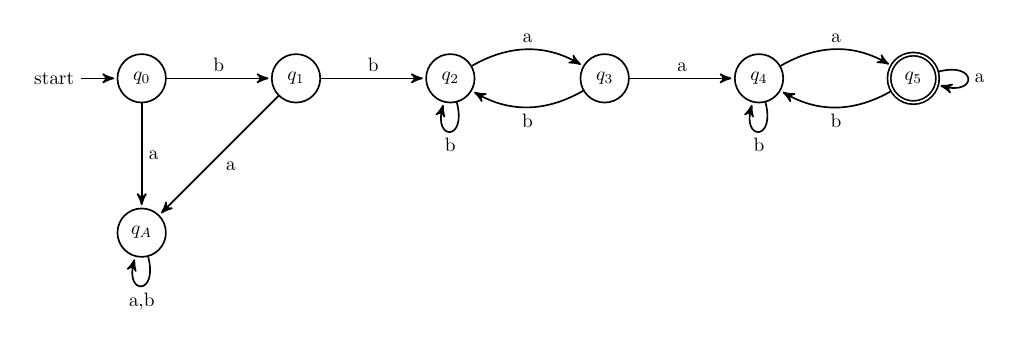
\begin{tikzpicture}[->,>=stealth',shorten >=1pt,auto,node distance=2.8cm,
                    semithick,every node/.style={scale=0.7}]
  \tikzstyle{every state}=[circle,text=black]

  \node[initial,state] 			(A)             	{$q_0$};
  \node[state]					(B) [right of=A]	{$q_1$};
  \node[state]					(C) [right of=B]	{$q_2$};
  \node[state]        			(D) [right of=C]	{$q_3$};
  \node[state]        			(E) [right of=D]	{$q_4$};
  \node[state,accepting]		(F) [right of=E]	{$q_5$};
  \node[state]        			(G) [below of=A]	{$q_A$};

  \path (A)	edge				node {a}	(G)
  			edge 				node {b}	(B)
  		(B)	edge 				node {a}	(G)
			edge 				node {b}	(C)
  		(C)	edge [bend left]	node {a}	(D)
  			edge [loop below]	node {b}	(C)
  		(D)	edge				node {a}	(E)
  			edge [bend left]	node {b}	(C)
  		(E)	edge [bend left]	node {a}	(F)
  			edge [loop below]	node {b}	(E)
 		(F)	edge [loop right]	node {a}	(F)
	  		edge [bend left]	node {b}	(E)
  		(G)	edge [loop below]	node {a,b}	(G)
  ;
\end{tikzpicture}
\end{center}

Die Klassen seiner Zustände sind:
\begin{enumerate}[\quad]
\item Kl[$q_0$] = $\{\lambda\}$
\item Kl[$q_1$] = $\{b\}$
\item Kl[$q_2$] = $\{bbx \mid x \in \{b,ab\}^*\}$
\item Kl[$q_3$] = $\{bbxa \mid x \in \{b,ab\}^*\}$
\item Kl[$q_4$] = $\{bbxaay \mid x \in \{b,ab\}^*, y \in \{a,b\}^*\}$
\item Kl[$q_5$] = $\{bbxaaya \mid x \in \{b,ab\}^*, y \in \{a,b\}^*\} = \{bbxa \mid x \in \{a,b\}^*$ und $x$ enthält das Teilwort $aa\}$
\item Kl[$q_A$] = $\{ax \mid x \in \{a,b\}^*\}$
\end{enumerate}

\end{enumerate}
\end{homeworkProblem}

\begin{homeworkProblem}
\begin{enumerate}[(a)]

\item
Der folgende endliche Automat akzeptiert nur Wörter $w$, für die $|w|_b$ mod $3 = 2$ gilt:

\begin{center}
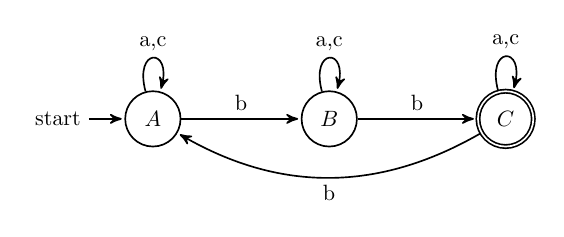
\begin{tikzpicture}[->,>=stealth',shorten >=1pt,auto,node distance=2.8cm,
                    semithick,every node/.style={scale=0.8}]
  \tikzstyle{every state}=[circle,text=black]

	\node[initial,state] 			(A)             	{$A$};
	\node[state]					(B) [right of=A]	{$B$};
	\node[state,accepting]			(C) [right of=B]	{$C$};

	\path	(A)		edge [loop above]		node {a,c}	(A)
	 				edge 					node {b}	(B)
	 		(B)		edge [loop above]		node {a,c}	(B)
	 				edge 					node {b}	(C)
			(C)		edge [loop above]		node {a,c}	(C)
	 				edge [bend left]		node {b}	(A)
  ;
\end{tikzpicture}
\end{center}



Es ist klar, dass $a$ und $c$ die Anzahl von $|w|_b$ nicht ändern und daher zu keiner Zustandsänderung führen. Für die Klassen gilt also:
\begin{enumerate}[\quad]
\item Kl[A] = $\{w \mid |w|_b$ mod $3 = 0\}$
\item Kl[B] = $\{w \mid |w|_b$ mod $3 = 1\}$
\item Kl[C] = $\{w \mid |w|_b$ mod $3 = 2\}$
\end{enumerate}

Der endliche Automat, der Wörter der Form $w=cxcyc$ für $x,y \in \{a,b\}^*$ akzeptiert, sieht folgendermassen aus:

\begin{center}
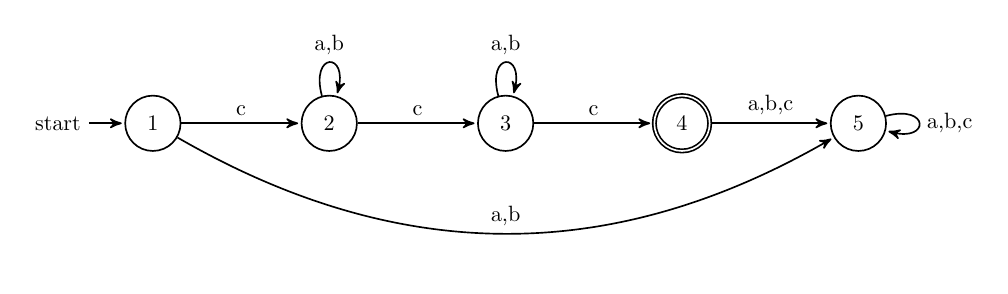
\begin{tikzpicture}[->,>=stealth',shorten >=1pt,auto,node distance=2.8cm,
                    semithick,every node/.style={scale=0.8}]
  \tikzstyle{every state}=[circle,text=black]

	\node[initial,state] 			(1)             	{$1$};
	\node[state]					(2) [right of=1]	{$2$};
	\node[state]					(3) [right of=2]	{$3$};
	\node[state,accepting]			(4) [right of=3]	{$4$};
	\node[state]					(5) [right of=4]	{$5$};

	\path	(1)		edge [bend right]		node {a,b}	(5)
	 				edge 					node {c}	(2)
	 		(2)		edge [loop above]		node {a,b}	(2)
	 				edge 					node {c}	(3)
			(3)		edge [loop above]		node {a,b}	(3)
	 				edge 					node {c}	(4)
			(4)		edge					node {a,b,c}(5)
			(5)		edge [loop right]		node {a,b,c}(5)
  ;
\end{tikzpicture}
\end{center}

Die Klassen sind:
\begin{enumerate}[\quad]
\item Kl[1] = $\{\lambda\}$
\item Kl[2] = $\{cx \mid x \in \{a,b\}^*\}$
\item Kl[3] = $\{cxcy \mid x,y \in \{a,b\}^*\}$
\item Kl[4] = $\{cxcyc \mid x,y \in \{a,b\}^*\}$
\item Kl[5] = $\{xy \mid x \in \{a,b\}, y \in \{a,b,c\}^*\}$
\end{enumerate}

Die beiden endlichen Automaten können nach der Methode des modularen Entwurfs (Konstruktion eines Produktautomaten) zu folgendem EA kombiniert werden. (Da im resultierenden EA die Zustände B1 und C1 nie erreicht werden können, löschen wir diese. Zusätzlich können die Zustände A5, B5 und C5 in einen kombiniert werden. So bleibt der EA übersichtlich.)

\begin{center}
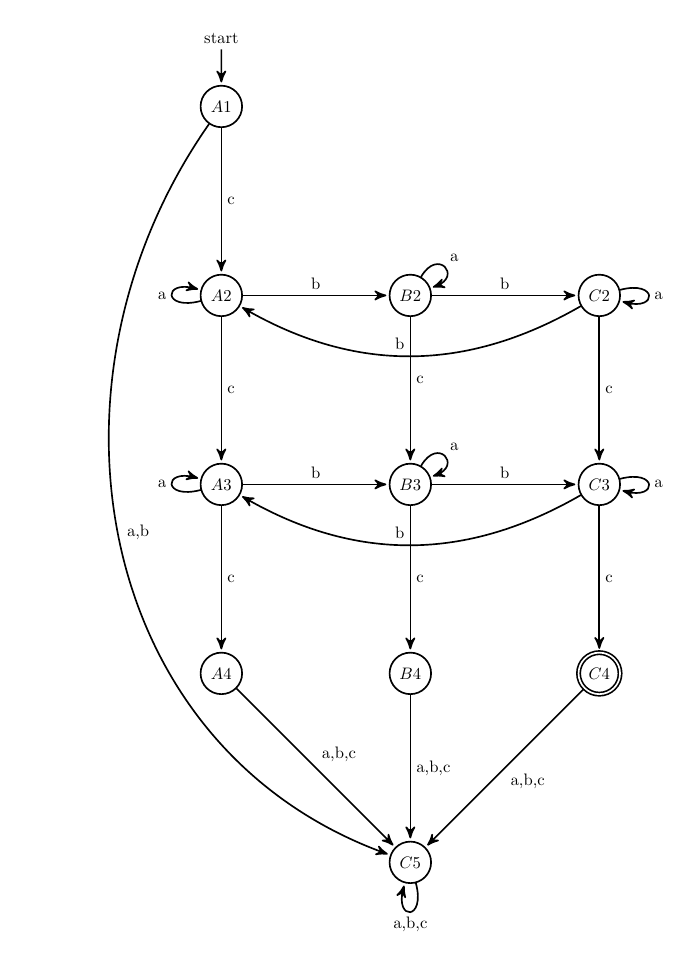
\begin{tikzpicture}[->,>=stealth',shorten >=1pt,auto,node distance=4cm,
                    semithick,every node/.style={scale=0.6}]
  \tikzstyle{every state}=[circle,text=black]

	\node[initial above,state]		(A1)             	{$A1$};
	\node[state]					(A2) [below of=A1]	{$A2$};
	\node[state]					(A3) [below of=A2]	{$A3$};
	\node[state]      			 	(A4) [below of=A3]	{$A4$};
	\node[state]					(B2) [right of=A2]	{$B2$};
	\node[state]					(B3) [below of=B2]	{$B3$};
	\node[state]      			 	(B4) [below of=B3]	{$B4$};
	\node[state]					(C2) [right of=B2]	{$C2$};
	\node[state]					(C3) [below of=C2]	{$C3$};
	\node[state,accepting]     	 	(C4) [below of=C3]	{$C4$};
	\node[state]        			(C5) [below of=B4]	{$C5$};
	
	\path	(A1)	edge 									node {c}	(A2)
			(A1)	edge [out=235,in=160,distance=4cm]		node {a,b}	(C5)
			(A2)	edge [loop left]						node {a}	(A2)
			(A2)	edge									node {b}	(B2)
			(A2)	edge 									node {c}	(A3)
			(A3)	edge [loop left]						node {a}	(A3)
			(A3)	edge									node {b}	(B3)
			(A3)	edge 									node {c}	(A4)
			(A4)	edge 									node {a,b,c}(C5)
			(B2)	edge [loop,out=60,in=20,looseness=6]	node {a}	(B2)
			(B2)	edge									node {b}	(C2)
			(B2)	edge [above right]						node {c}	(B3)
			(B3)	edge [loop,out=60,in=20,looseness=6]	node {a}	(B3)
			(B3)	edge									node {b}	(C3)
			(B3)	edge 									node {c}	(B4)
			(B4)	edge 									node {a,b,c}(C5)
			(C2)	edge [loop right]						node {a}	(C2)
			(C2)	edge [bend left=30,above left]			node {b}	(A2)
			(C2)	edge 									node {c}	(C3)
			(C3)	edge [loop right]						node {a}	(C3)
			(C3)	edge [bend left=30,above left]			node {b}	(A3)
			(C3)	edge 									node {c}	(C4)
			(C4)	edge 									node {a,b,c}(C5)
			(C5)	edge [loop below]						node {a,b,c}(C5)
  ;
\end{tikzpicture}
\end{center}

\item
asdf

\end{enumerate}
\end{homeworkProblem}

\begin{homeworkProblem}
\begin{enumerate}[(a)]

\item
$L_1=\{0^m1^n0^{m+n}\,|\,m, n \in \mathbb{N}\}$\\
Annahme: Sei $L_1$ regulär. Dann gibt es einen endlichen Automaten $A=(Q,\,\Sigma,\,\delta_A,\,q_0,\,F)$, sodass $L(A)=L$. Dieser hat $|Q_0|$ Zustände. Nach dem \textit{Pumping-Lemma} lässt sich ein $w$ mit $|w|=n_0$ in $w=xyz$ zerlegen und
\begin{enumerate}[(i)]
\item $|yx| \leq n_0$
\item $|x| \geq 1$
\item $\{yx^kz\,|\,k\in\mathbb{N}\} \subseteq L \quad\text{oder}\quad \{yx^kz\,|\,k\in\mathbb{N}\} \cup L = \emptyset$
\end{enumerate}
Jedes Wort $w$ der Länge $|w| \geq n_0$ muss also eine Zerlegung besitzen, die (i), (ii), (iii) erfüllt.\\
Sei $W=1^{n_0}0^{n_0}$, also $|w|=2*n \geq n_0$
\begin{align*}
\text{(i)}&\Rightarrow y=1^l,\;x=1^m\quad \text{mit }l,\,m \in \mathbb{N}\\
\text{(iii)}&\Rightarrow \text{Da } w=1^{n_0}0^{n_0}\in L, \text{ ist } \{yx^kz\,|\,k\in\mathbb{N}\}=\{1^l\left(1^m\right)^k0^{n_0}\} \subseteq L 
\end{align*}
Aber: für $k=0$ ist $w=yz=1^{n_0-m}0^{n_0} \not\in L$\\
Wir haben einen Widerspruch, daher war die Annahme, dass L regulär ist, falsch.

\item
Wir machen einen Widerspruchsbeweis. Annahme: $L$ ist regulär. \\Dann gilt das \textit{Pumping-Lemma} auch für $L$.\\
Betrachten wir das Wort $0^{{n_0}^2+n_0}$, dann ist offensichtlich $|w| \geq n_0$\\
Für alle Zerlegungen $w=yxz$ gilt
\[ y=0^l,\,x=0^m,\,z=0^{{n_0}^2+n_0-l-m} \quad\text{mit}\quad |xy|\leq n_0 \quad\text{und}\quad |x|\geq 1
\]\\
\\Weil $w=yxz=0^{{n_0}^2+n_0}\in L$, muss $yx^kz\in L$ erfüllt sein.\\
\\Es gilt aber: 
\[
yx^2z=0^l0^{2m}0^{{n_0}^2+n_0-l-m}=0^{{n_0}^2+n_0+m}\not\in L\quad,
\]
weil
\[
{n_0}^2+n_0\leq{{n_0}^2}+n_0+m\leq {n_0}^2+3n_0+2=(n_0+1)(n_0+2)
\]
\[
{{n_0}^2}+n_0+m \quad\text{hat also nicht die Form}\quad n(n+1)
\]
\\ 
Wir haben nun ein Widerspruch, womit die Annahme, dass L eine reguläre Sprache ist, verworfen wird.
\end{enumerate}
\end{homeworkProblem}

\end{document}
